\documentclass[conference,onecolumn,12pt]{IEEEtran}
\IEEEoverridecommandlockouts
\hyphenation{op-tical net-works semi-conduc-tor}
\usepackage{fancyhdr}
\usepackage{lipsum}
\usepackage{amsmath,amssymb,amsfonts}
\usepackage{algorithmic}
\usepackage{graphicx}
\usepackage{textcomp}
\usepackage{comment}
\usepackage{xcolor}
\usepackage{float}
\usepackage{svg}
\usepackage{tabularx}
\usepackage{hyperref}
\usepackage{breqn}
\usepackage{makecell}
\usepackage{siunitx}
\usepackage{hyperref}
\usepackage{multirow}
\usepackage{booktabs}
\usepackage{stfloats}

\usepackage[style=numeric]{biblatex}  % Choose a style like numeric, authoryear, etc.
\addbibresource{references.bib}       % Note: use this instead of \bibliography

\defbibheading{bibliography}[\bibname]{\section*{Referencias}}

%\usepackage{circuitikz}

%\addbibresource{references.bib}
\renewcommand{\IEEEkeywordsname}{Palabras Clave}
\renewcommand{\tablename}{Tabla} 
\renewcommand{\abstractname}{Resumen} 
\renewcommand{\figurename}{Fig.}
\numberwithin{equation}{subsection}


%-------------------------No tocar de aqui para atras-----------

%-------------------------Título y nombres-----------
\begin{document}

\title{Tarea 2. Teoría de la información: \\Códigos de Huffman}
\author{
\IEEEauthorblockN{
Fabián Alonso Gómez Quesada\IEEEauthorrefmark{1}, Wilberth Daniel Gutiérrez Montero\IEEEauthorrefmark{2} \\
Nagel Eduardo Mejía Segura\IEEEauthorrefmark{3}, Oscar Mario González Cambronero\IEEEauthorrefmark{4}
}
\IEEEauthorblockA{
\IEEEauthorrefmark{1}\IEEEauthorrefmark{2}\IEEEauthorrefmark{3}\IEEEauthorrefmark{4} Escuela de Ingeniería en Electrónica, Instituto Tecnológico de Costa Rica. \\
\small Emails: fabi.goque@estudiantec.cr, wil.gutierrez@estudiantec.cr,\\ nagelmese@estudiantec.cr, oscargonzalezc@estudiantec.cr
}
}


\maketitle
\thispagestyle{plain}
\pagestyle{plain}
%------- %-------------------------Inicio----------- 

\begin{abstract} 

El presente informe expone la aplicación de los códigos de Huffman dentro del marco de la teoría de la información, a través de una serie de experimentos con códigos de programación junto a archivos de texto e imagen, con el fin de explorar conceptos como entropía, eficiencia de codificación, compresión sin pérdida y reconstrucción de datos. El lenguaje utilizado para el experimento es Python, que permite implementar el algoritmo de Huffman, calcular métricas estadísticas y comparar la codificación original del archivo con codificación generada.

\end{abstract} 
%-------------------------Palabras clave-----------
\begin{IEEEkeywords} Codificación, entropía, Huffman, Python.
\end{IEEEkeywords} 

\section{Introducción}

La teoría de la información constituye una base fundamental en el estudio de sistemas de comunicación. Dentro de este campo, los códigos de Huffman se destacan como una técnica eficiente para la compresión sin pérdida de datos, eliminando redundancias presentes en las fuentes de información. El objetivo del presente informe es explorar de manera práctica los conceptos relacionados con la entropía, la codificación eficiente y la reconstrucción de datos utilizando códigos de Huffman. A partir de la implementación en Python de dicho algoritmo, se analizará su rendimiento sobre distintos tipos de datos, se evaluará la eficiencia comparada con la codificación original, y se examinará cómo la entropía de una fuente afecta la compresibilidad de sus datos. 

\section{Desarrollo del proyecto}

\subsection{Algoritmo de Huffman}

\subsubsection{Implementación del código de Huffman}
\hfill\break 

\textbf{¿Cómo se implementa el algoritmo de generación de códigos Huffman?}


El script “huffman base.py” comienza recibiendo instrucciones desde la línea de comandos a través de la función myfunc(argv), la cual se encarga de interpretar los argumentos para identificar el archivo de entrada, cuya ruta debe ser proporcionada por el usuario. A continuación, se definen las rutas y nombres para los archivos: comprimido, diccionario y descomprimido. Posteriormente, el archivo original sin comprimir se lee byte por byte en modo binario y su contenido se almacena en una cadena de texto. Seguidamente, se implementan funciones relacionadas con la creación y manipulación del árbol binario utilizado en el proceso de compresión de Huffman. Una vez construido el árbol y sus nodos, se recorre para asignar un código binario a cada símbolo, el cual se guarda en un diccionario que enlaza símbolos con sus respectivos códigos.
\\
\\
\textbf{¿Cómo están codificados los datos del archivo solo\textunderscore abc\textunderscore cien.txt? ¿Cuántos bits se usan para representar cada carácter? ¿Qué espera observar al correr el algoritmo de Huffman?}

El archivo de prueba solo_abc_cien.txt contiene múltiples repeticiones de las letras de la “A” a la “Z”, específicamente 100 veces cada una, lo que hace que todos los símbolos tengan una probabilidad de aparición similar. Los datos están codificados en formato ASCII bajo el estándar UTF-8, lo cual implica que cada carácter ocupa 8 bits. Aunque UTF-8 permite longitudes variables por carácter, en este caso se emplea una codificación fija de 1 byte (8 bits) por símbolo. Al aplicar el algoritmo de Huffman sobre este archivo, se espera que los caracteres más frecuentes se codifiquen con menos bits; sin embargo, dado que todos los símbolos tienen la misma frecuencia, es razonable anticipar que las longitudes de los códigos resultantes sean muy similares entre sí. En consecuencia, la varianza del código generado será baja y el diccionario Huffman mostrará una tabla donde cada símbolo estará asociado a un código binario de longitud comparable.
\\
\\
\textbf{¿Cuáles son sus observaciones al ejecutar el código sobre el archivo llamado solo\textunderscore abc\textunderscore cien.txt?}

Al correr el código con dicho archivo, se obtiene la Tabla \ref{tab:huffman_abc} donde se observa que la mayoría de códigos tienen 5 bits, con excepción de 6 simbolos que contemplan 4 bits.

\begin{table}[h!]
    \centering
    \caption{Códigos Huffman para caracteres ASCII (A-Z)}
    \label{tab:huffman_abc}
    \begin{tabular}{ccc}
    \toprule
    \textbf{Char (decimal)} & \textbf{Símbolo} & \textbf{Código Huffman} \\
    \midrule
    65 & A & 0001 \\
    66 & B & 0000 \\
    67 & C & 0011 \\
    68 & D & 0010 \\
    69 & E & 10101 \\
    70 & F & 10100 \\
    71 & G & 10111 \\
    72 & H & 10110 \\
    73 & I & 10001 \\
    74 & J & 10000 \\
    75 & K & 10011 \\
    76 & L & 10010 \\
    77 & M & 11101 \\
    78 & N & 11100 \\
    79 & O & 11111 \\
    80 & P & 11110 \\
    81 & Q & 11001 \\
    82 & R & 11000 \\
    83 & S & 11011 \\
    84 & T & 11010 \\
    85 & U & 01101 \\
    86 & V & 01100 \\
    87 & W & 01111 \\
    88 & X & 01110 \\
    89 & Y & 0101 \\
    90 & Z & 0100 \\
    \bottomrule
    \end{tabular}
\end{table}

\subsubsection{Hipotesis de Archivos}
\hfill\break 

\begin{itemize}
    \item \textbf{todo\_ascii\_cien.bin}: El archivo consiste de los 256 códigos para ASCII repetidos 100 veces, por lo tanto, cada simbolo es equiprobable, la entropía sería igual a $\log_2(8)$, si bien los códigos van a cambiar por como está programado el código de huffman, sin embargo, la longitud del código se mantiene en 8 bits. La eficiencia no cambia con el código nuevo.
    \item \textbf{shannon\_intro.txt}: El archivo contiene texto relacionado con los fundamentos teóricos de la comunicación, posiblemente basado en los trabajos de teoría de Claude Shannon. En él se aborda cómo cuantificar la información transmitida en un sistema de comunicación y cómo diferentes esquemas de modulación, como PCM (modulación por pulsos codificados) y PPM (modulación por posición de pulsos), logran intercambiar ancho de banda por mejoras en la relación señal/ruido. Al aplicar el algoritmo de Huffman sobre este archivo, se espera que se asignen códigos de longitud variable a los caracteres, donde aquellos que aparecen con mayor frecuencia reciban códigos más cortos. Esto se traduce en una codificación más eficiente al reducir la longitud promedio del código.
    \item \textbf{h\_cero.bin}: El archivo contiene exclusivamente la letra "H" repetida a lo largo de todo el archivo. Al tratarse de una fuente con un único símbolo, la entropía es mínima (cero en teoría), y el código de Huffman asignado será extremadamente simple: bastará con un solo bit para representar toda la información. En este caso, la longitud promedio del código también será mínima y la eficiencia será del 100%, ya que no existe redundancia adicional que pueda ser explotada.
    \item \textbf{4.1.01.tiff}: Corresponde a una imagen. En este caso, el análisis del contenido se realiza a nivel de bits, y la compresión mediante Huffman depende en gran medida del nivel de redundancia presente en los patrones binarios de la imagen. En este caso se muestra una persona y hay gran variación de colores en la imagen.
    \item \textbf{4.2.03.tiff}: Es una imagen, que muestra un mandril con gran variedad de colores, lo que implica una alta diversidad de valores de píxeles. Desde el punto de vista de la teoría de la información, esto se traduce en una alta entropía, ya que hay poca redundancia en los datos. Al aplicar Huffman, la longitud promedio del código tenderá a ser mayor, ya que los símbolos tienen probabilidades más uniformes y se requiere más información para representarlos. En consecuencia, la eficiencia de compresión será menor comparada con imágenes más simples o menos variadas, ya que hay menos redundancia que explotar.
    \item \textbf{5.1.11.tiff}: Es una imagen, que muestra un avión en escala de grises, lo que reduce considerablemente la cantidad de colores posibles. Esto puede generar mayor redundancia en los datos, por tanto, la entropía es moderada, y el algoritmo de Huffman puede asignar códigos más cortos a los valores de gris más frecuentes. Se espera una longitud promedio del código menor que en imágenes a color, y una eficiencia de codificación aceptable.
    \item \textbf{5.1.13.tiff}: Es una imagen, que muestra un fondo blanco con patrones de polígonos, números en negro y algunos grises. Debido a su simplicidad y contraste marcado entre pocos tonos, presenta una baja entropía, ya que la mayoría de los píxeles corresponden al fondo blanco. En este escenario, Huffman puede asignar códigos muy cortos a los símbolos más comunes, como el blanco, y más largos a los símbolos menos frecuentes. Esto se traduce en una longitud de código promedio baja y una alta eficiencia de compresión, ya que el algoritmo aprovecha al máximo la redundancia presente.
    \item \textbf{7.1.02.tiff}: Es una imagen, que muestra en escala de grises un jet en tierra, donde la reducción en la paleta de colores disminuye la entropía respecto a una imagen a color. La longitud promedio del código depende de la distribución de tonos, pero se espera moderada, y la eficiencia se espera sea buena ya que predominan algunos tonos de grises en grandes áreas.
\end{itemize}

\subsubsection{Resultados obtenidos}

Se realizó la modificación al script para obtener algunos parámetros como la entropía, la longitud media, varianza, eficiencia de la codificación original y eficiencia del nuevo código generado. En la Fig. \ref{fig:modscript} se observa la modificación al script para el cálculo de los parámetros requeridos.

\begin{figure}[!h]
    \begin{center}
        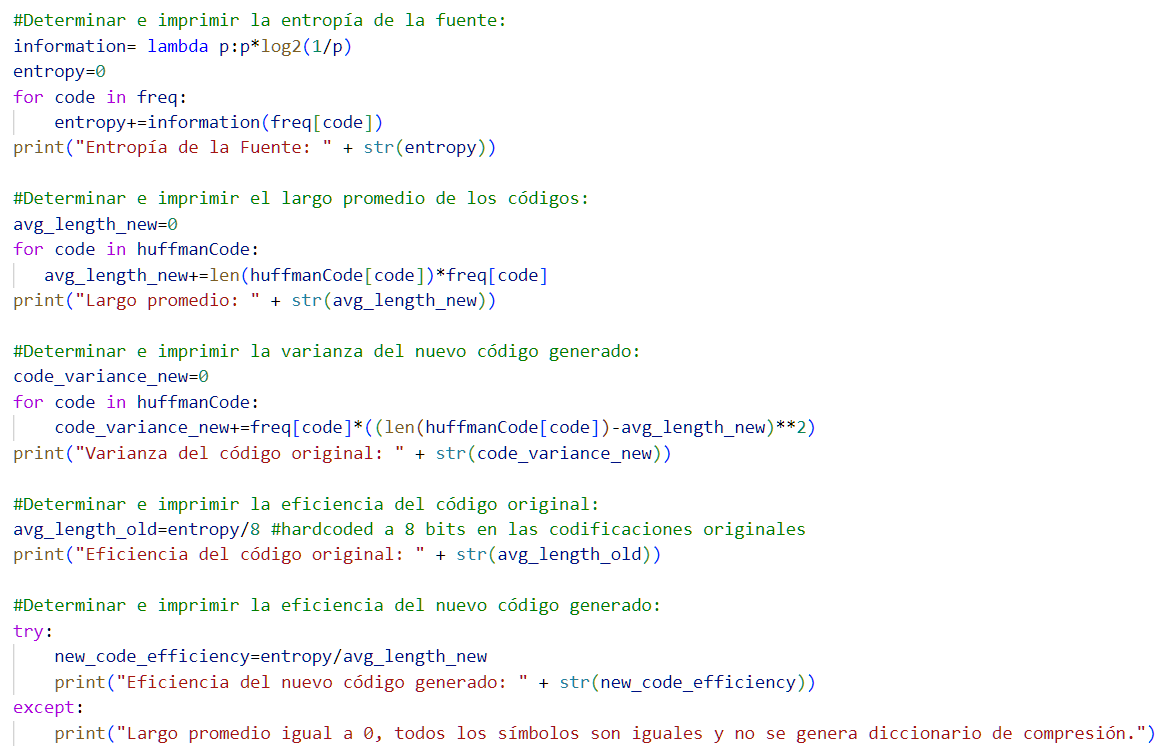
\includegraphics[width=0.9\linewidth]{figures/modscript.png}
        \caption{Modificación del script para el cálculo de nuevos parámetros}
        \label{fig:modscript}
    \end{center}
\end{figure}

En la Tabla \ref{tab:huffman_resultados} se observan los resultados al ejecutar el script con todos los archivos mostrados.

\hfill\break \hfill\break \hfill\break \hfill\break \hfill\break
\hfill\break 


 \begin{table*}[h!]
    \centering
    \caption{Resultados de codificación Huffman sobre distintos archivos.}
    \label{tab:huffman_resultados}
    \begin{tabular}{lccccc}
    \toprule
    \textbf{Archivo} & \textbf{Entropía} & \textbf{Largo Promedio} & \textbf{Varianza} & \textbf{Efic. Código Orig.} & \textbf{Efic. Código Gen.} \\
    \midrule
    todo\_ascii\_cien.bin & 8.00 & 8.00 & 3.16e-30 & 1.00 & 1.00 \\
    shannon\_intro.txt & 4.37 & 4.40 & 2.08 & 0.55 & 0.99 \\
    h\_cero.bin & 0.00 & 0.00 & 0.00 & 0.00 & - \\
    4.1.01.tiff & 6.90 & 6.93 & 1.01 & 0.863 & 0.996 \\
    4.2.03.tiff & 7.76 & 7.80 & 0.607 & 0.970 & 0.995 \\
    5.1.11.tiff & 6.46 & 6.48 & 2.27 & 0.808 & 0.997 \\
    5.1.13.tiff & 1.57 & 1.95 & 6.32 & 0.196 & 0.803 \\
    7.1.02.tiff & 4.01 & 4.06 & 3.68 & 0.501 & 0.989 \\
    \bottomrule
    \end{tabular}
\end{table*}

\begin{itemize}
    \item \textbf{todo\_ascii\_cien.bin}: En este caso se observa que la entropía y la longitud promedio son de exactamente 8 bits, lo que se alinea con una codificación ASCII de 256 símbolos equiprobables, la eficiencia original y generada son ambas de 1, lo que es coherente ya que no hay redundancia que comprimir.
    
    \item \textbf{shannon\_intro.txt}: La entropía indica una fuente con distribución de símbolos desigual, pero al ser la longitud promedio muy cercana a la entropía, sugiere que la codificación fue eficiente. La varianza muestra una distribución dispersa de las longitudes del código, lo cual es consistente con un texto donde caracteres como espacios o vocales son más frecuentes. La eficiencia original y la del código generado evidencian que hay una mejora significativa al utilizar Huffman.
    
    \item \textbf{h\_cero.bin}: Al contener un único símbolo, se esperaba y se obtuvo una entropía de 0, al igual que la longitud del código. La eficiencia del código original es 0, porque usar más de un bit para un símbolo único es completamente redundante. No se reporta eficiencia generada porque no hay nada que codificar.  
    
    \item \textbf{4.1.01.tiff}: La imagen tiene entropía moderadamente alta y longitud promedio muy cercana a la entropía. La eficiencia del código generado es casi 1, indicando que Huffman está aprovechando bien las frecuencias relativas.
    
    \item \textbf{4.2.03.tiff}: Presenta una entropía y longitud promedio muy similar, como era de esperarse para una imagen con gran variabilidad de colores. La eficiencia del código generado es alta, aunque la eficiencia original también es bastante buena, reflejando que el archivo original ya está optimizado.
    
    \item \textbf{5.1.11.tiff}:  Presenta entropía moderada y longitud muy similar, con una varianza considerable, lo cual puede deberse a que ciertos tonos se repiten más que otros. La eficiencia generada es muy alta, mostrando un uso efectivo del algoritmo.
    
    \item \textbf{5.1.13.tiff}: La entropía es muy baja, lo que concuerda con la gran cantidad de fondo blanco. La longitud del código no está tan cercana a la entropía, y la varianza es alta, probablemente porque algunos símbolos menos frecuentes recibieron códigos largos. La eficiencia generada es notablemente baja, pero esto es esperable dado el contraste fuerte entre frecuencias muy distintas y aún así es mejor que la eficiencia original.
    
    \item \textbf{7.1.02.tiff}: Muestra una entropía baja con longitud promedio muy cercana y varianza relativamente alta, indicando diferencias notables entre la frecuencia de los tonos. La eficiencia del código generado es bastante alta , aunque la original sea baja, evidenciando una mejora significativa mediante Huffman.
    
\end{itemize}

\subsection{Compresión por medio del código de Huffman}

\subsection{Restablecimiento de los datos originales - Descompresión}

\subsection{Efecto de la entropía de la fuente}

\section{Conclusiones} 

\begin{itemize}

\item Se comprobó 

\item El 

\item Se demostró 

\item  En cuanto

\end{itemize}


\section{Referencias Bibliográficas}
\printbibliography[heading=none]

\section{Anexos}

\href{https://github.com/NagelMS/Tarea2_CE2.git}{Link al repositorio de GitHub}

\end{document} 

 

 

 
